% !TEX program = XeLaTeX
% !TEX encoding = UTF-8
\documentclass[UTF8]{ctexart}
%{ctexart}


%\setCJKmainfont[BoldFont=FandolSong-Bold.otf,ItalicFont=FandolKai-Regular.otf]{FandolSong-Regular.otf}
%\setCJKsansfont[BoldFont=FandolHei-Bold.otf]{FandolHei-Regular.otf}
%\setCJKmonofont{FandolFang-Regular.otf}

\usepackage{url}
\usepackage{cancel}
\usepackage{xspace}
\usepackage{graphicx}
\usepackage{multicol}
\usepackage{multirow}
\usepackage{subfig}
\usepackage{amsmath}
\usepackage{amssymb}
\usepackage[a4paper, width=186mm, top=18mm, bottom=18mm, includeheadfoot]{geometry}
%\usepackage[a4paper, width=140mm, top=18mm, bottom=22mm, includeheadfoot]{geometry}
\usepackage{booktabs}
\usepackage{array}
\usepackage{verbatim}
\usepackage{caption}
\usepackage{natbib}
\usepackage{booktabs}
\usepackage{float}
\usepackage{pdflscape}
\usepackage{mathtools}
\usepackage[usenames, dvipsnames]{xcolor}
\usepackage{afterpage}
\usepackage{pgf}
\usepackage{tikz}
\usepackage{dirtree}
\usepackage[style=american]{csquotes}
\usepackage{amsfonts}
\usepackage{tikz}
\usepackage{tkz-graph}
\usetikzlibrary{arrows,decorations.pathmorphing,automata,positioning,backgrounds,fit,shapes.symbols,chains,intersections}

\newtheorem{definition}{定义}[section]
\newtheorem{theorem}{Theorem}[section]
\newtheorem{lemma}{Lemma}
\newtheorem{proof}{Proof} [section]



\usepackage[toc, page, title, titletoc, header]{appendix}
\usepackage{marginnote}
\usepackage{tablefootnote}

\renewcommand\appendixname{附\ 录}
\renewcommand\appendixpagename{附\ 录}
\renewcommand\appendixtocname{附\ 录}
\renewcommand\abstractname{摘要}


\usepackage{perpage} %the perpage package
\MakePerPage{footnote} %the perpage package command

\usetikzlibrary{shapes.geometric}%
\usepackage{color}
%\usepackage[pages=some, placement=top]{background}
\usepackage{eso-pic}
\usepackage[final]{pdfpages}

%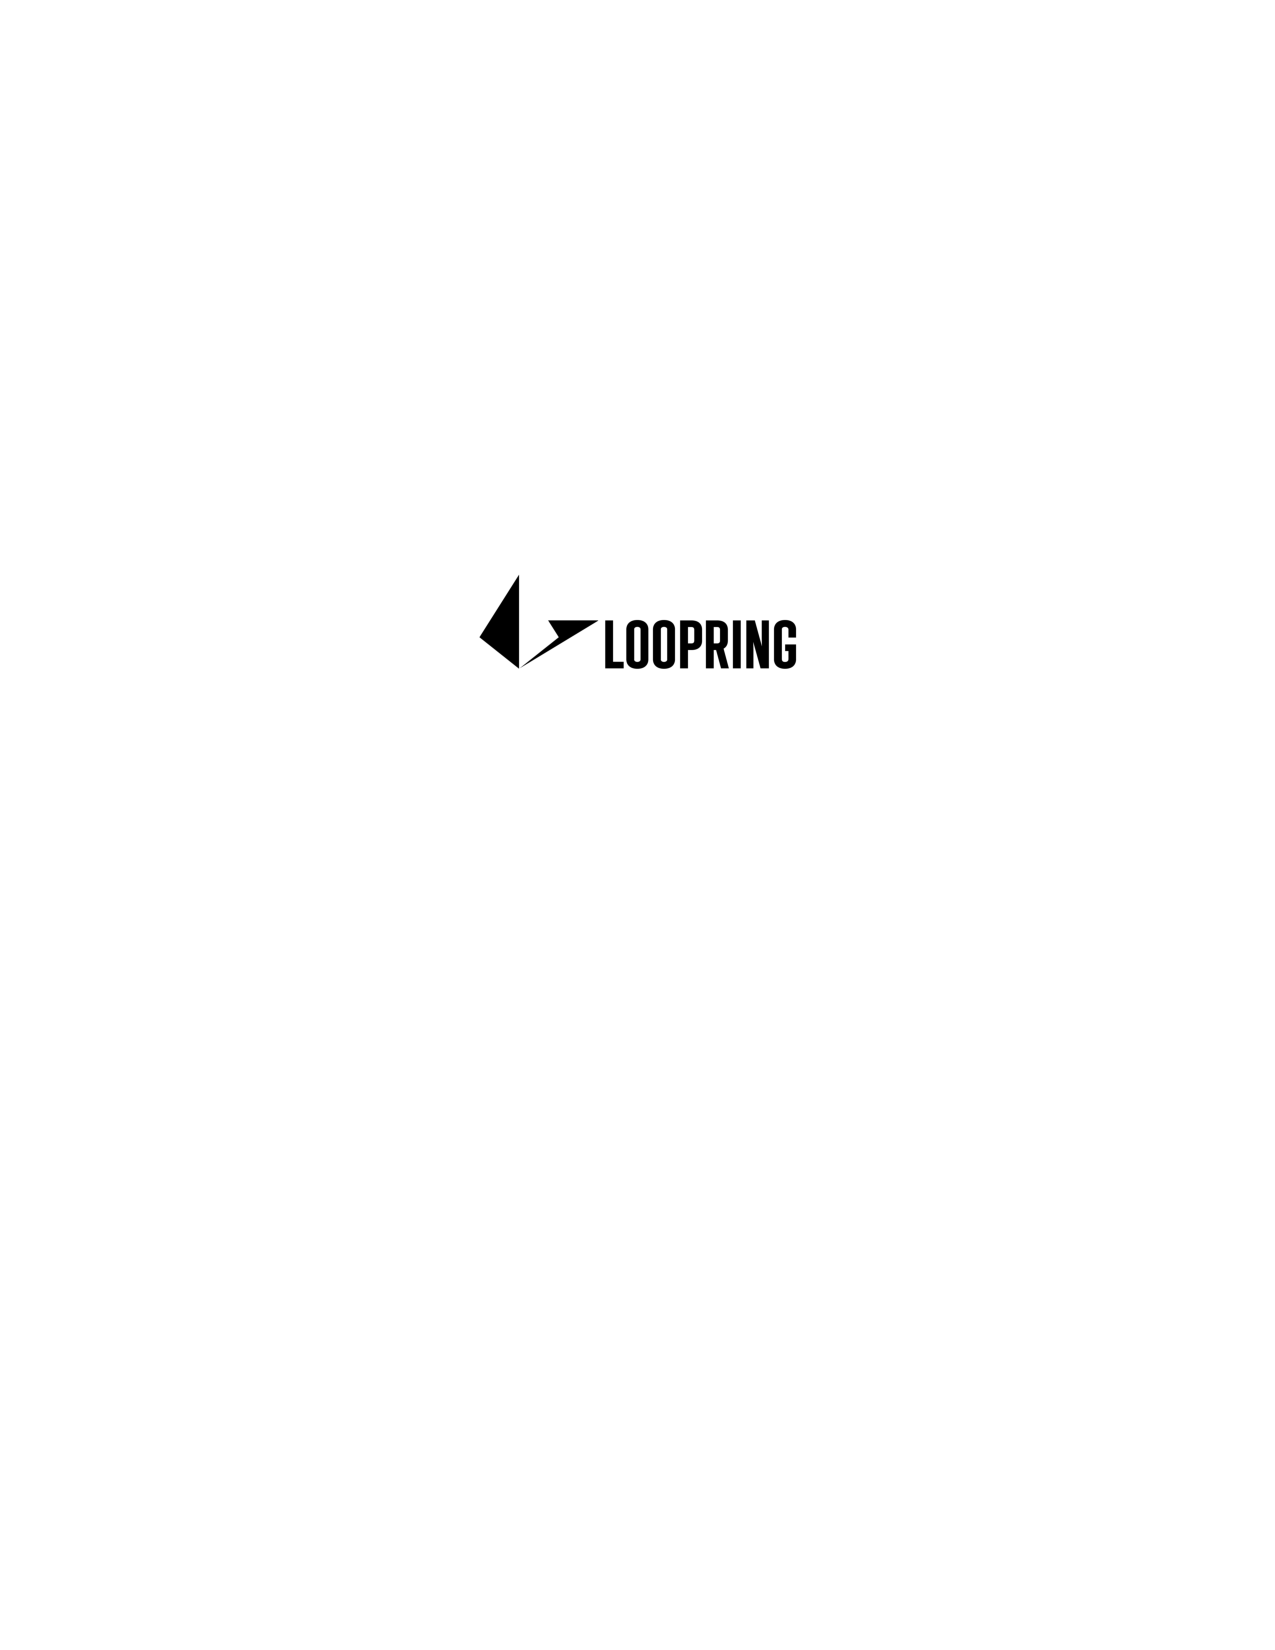
\includepdf[pages=1]{cover}
\hyphenpenalty=750

\title{\textbf{LOOPRING(路印):}\\\textbf{去中心化代币交易撮合协议}}
\author{
  王东\\
  \texttt{daniel@loopring.org}\\
  \and
  	周杰\\
  	\texttt{jay@loopring.org}\\
  	\and
  	王辉\\
  	\texttt{alex@loopring.org}\\
  	\and
  	Matthew Finestone\\
  	\texttt{matt.finestone@gmail.com}\\ 
  \\
  \texttt{https://loopring.org}
 }

\makeatletter
\def\CTEX@section@format{\Large\bfseries}
\makeatother

\makeatletter
\newenvironment{tablehere}
 {\def\@captype{table}}
 {}

\newenvironment{figurehere}
 {\def\@captype{figure}}
 {}
\makeatother
%
%\newcommand\BackgroundPic{%
%\put(0, 0){%
%\parbox[b][\paperheight]{\paperwidth}{%
%\vfill
%\centering
%\includegraphics[width=\paperwidth, height=\paperheight, %
%%keepaspectratio]{images/background.jpg}%
%]{images/background.jpg}%
%\vfill
%}}}


\begin{document}
%\AddToShipoutPicture{\BackgroundPic}
\maketitle


\begin{abstract}
路印是一种构建去中心化交易网络的开源协议,其不仅拥有一套公开的用于执行交易和撮合操作的智能合约,而且还有一组链下参与者用来撮合和广播订单。路印协议是免费、可扩展的,可以被看作是附带交易功能的去中心化应用(dApps)的标准构成要素。它的互操作标准促进了无需信任的匿名交易的实现。与当前现有的去中心化交易协议相比,路印带来的一个重要改进是能够将不同订单进行撮合、匹配,从而消除了两个代币交易对的约束,大大提高了流动性。此外,路印还部署了一套独特的防范抢先交易(一种不公平的,试图以比原始解决方案提供商更快的速度向区块提交交易的行为)的增强解决方案。另外,路印是区块链不可知的,可以部署到任何具备智能合约功能的区块链上。在本文撰写之时,路印协议已经在Ethereum(以太坊) \cite{buterin2017ethereum} \cite{wood2014ethereum} 和Qtum(量子链) \cite{dai2017smart} 上成功运行,在NEO \cite{atterlonn2018distributed} 上正在进行部署。
\end{abstract}



\begin{multicols}{2}
\section{简介\label{sec:introduction}}

随着区块链资产的激增,交易双方之间交换这些资产的需求大大增加。伴随着数以千计的新代币的出现——包括传统资产的代币化——这一需求又被放大了。无论是出于投机交易动机,还是想要通过交换来的原生应用代币实现接入网络的目的,对于更宏大的生态系统而言,实现加密数字货币资产之间的互换都是一项基本需求。事实上,这些资产 \cite{desotocapital}中存在着某种潜在的能量,将这种能力释放出来——解锁资本——不仅要求拥有资产所有权(区块链已经永久性地实现了这点),而且还需要让交易双方能够自由地转移和转换这些资产。
 
正因如此,无需信任的代币(价值)交易成为了区块链技术一个引人注目的使用案例。然而,直到如今,大多数加密数字货币爱好者依然满足于在传统的中心化交易所交易代币。因此市场对于路印协议的需要是迫切的,正如比特币 \cite{nakamoto2008bitcoin} 一直以来所强调的那样,对于点对点电子现金而言, \enquote{如果我们依然需要一个可信赖的第三方来防范‘双花’问题的发生,那么点对点现金对于我们而言就失去了优势}。同理,如果我们依然需要借助可信赖的、封闭的、中心化的交易所来交易去中心化资产,去中心化资产的显著特性也就不复存在了。

从哲学角度讲,在中心化交易所交易去中心化代币也根本说不通,因为其违背了这些去中心化项目所秉持的理念。此外,在下文中我们也详细描述了使用中心化交易所所面临的诸多风险和限制。一直以来, 去中心化交易 (DEXs) \cite{schuh2015bitshares} \cite{bancor} \cite{kyber} 也在试图解决这些问题,而且在许多情况下已经成功运用区块链技术去中介化的特点减轻了一些安全风险。然而,随着DEX的性能逐步成为新经济时代的重要基础设施,目前的DEX仍有很大的性能提升空间。路印的目的就是用其dApp不可知的开源协议为这些基础设施的构建提供模块化工具。

\section{当前交易所现状\label{sec:current_exchange_landscape}}

\subsection{中心化交易所存在的不足}
中心化交易所面临的三大主要风险是:1)缺乏安全性,2)缺乏透明度,3)缺乏流动性。

\textbf{缺乏安全性} 源于用户常常都是把自己的私钥(资金)交给一个中心化的实体来管理。这种做法使用户不得不面临中心化交易所成为恶意黑客攻击牺牲品的可能。不过,尽管大家都知道所有中心化交易所都面临安全和被黑客攻击的风险 \cite{coincheckhack}  \cite{mcmillan2014inside} ,但却常常把这种风险看作是一种代币交易的“入场筹码”。目前,中心化交易所仍然是黑客攻击的“蜜罐”,因为他们的服务器上保管着超过数百万美元的用户资金。此外,交易所开发人员在用户资金管理方面也可能会犯一些诚实、偶然的错误。简单地说,用户将代币充值到一家中心化交易所之后,这些代币就不再受他们控制了。

\textbf{缺乏透明度} 会让用户不公地面临交易所不正当行为所带来的风险,这里我们主要指的是交易所运营商的恶意行为。因为对于用户而言,实际上他们在中心化交易所交易的并不是自己的资产,而是IOU。代币发送到交易所钱包之后,便开始由交易所保管,然后其会为用户提供IOU记账。因此,用户之后的所有交易实际上是这些IOU之间的交易。提现时,用户会向交易所申请赎回他们的IOU,由交易所将相应代币发送至用户在交易所以往的钱包地址。整个过程缺乏透明,交易所有可能突然关闭,冻结你的帐户或者破产。此外,交易所还可能会将替用户保管的资产挪作他用,比如借给第三方。缺乏透明虽然可能不会造成用户损失全部资金,但有可能会带来较高的交易手续费,需求高峰期订单延迟,监管风险以及订单被抢先交易等风险。

\textbf{缺乏透明度} 从交易所运营商的角度看,碎片化的流动性会抑制新交易所的出现,因为有可能两家交易所就可以吃掉整个市场。首先是拥有交易对最多的交易所会取胜,因为用户想要在一家交易所操作自己所有的交易。其次是订单表深度最厚的交易所,因为每个交易对都存在着可观的买卖价差。这种情况会抑制新来者加入竞争,因为它们难以建立起初始流动性。这种现象带来的结果是很多交易所尽管用户抱怨颇多,或者甚至发生过重大黑客攻击事件,但却依然占有着较高的市场份额。值得注意的是,随着中心化交易所占的市场份额越高,成为更大的攻击目标的可能性就越大。

从用户的角度看,碎片化的流动性会大大影响用户体验,因为在中心化交易所,他们只能在交易所自身的流动池、订单表以及所支持的交易对中进行交易。想要用代币 \verb|A| 来交易代币 \verb|B|,用户必须选择一家同时支持这两种代币交易的交易所,或者在不同的交易所提供自己的个人信息,注册帐号。此外,用户常常需要执行一步初始或者中间交易,多数是对BTC或ETH交易对,并在这一过程中支付买卖价差。最后,如果不下调订单量,用户有可能由于订单表深度不够而无法完成交易。即使交易所声称自身可以承受大额交易,但依然不可以保证这些成交量和流动性不是伪造的 \cite{fakevolume}。

其结果是,流动性散落,生态系统支离破碎,类似于传统的金融体系,大量的交易量都集中在少数交易所。区块链的全球流动性承诺在中心化交易所中毫无价值。

\subsection{去中心化交易所存在的不足}
去中心化交易所与中心化交易所不同,部分原因是在去中心化交易所中,用户控制这他们的私钥(资产)在区块链上执行交易。通过利用加密货币自身无需信任的技术,它们成功地减少了许多上述提到的安全风险。然而,去中心化交易所依然存在着性能和结构限制等问题。

而且常常来讲,流动性依然是个问题,因为用户必须在不同的流动性资金池中寻找交易对手方。如果DEX或dApp不部署可互操作的统一标准,不能做到在一个更广的网络中分享/广播订单,流动性分割效应就依然存在。限价订单表的流动性,也就是弹性——被吃掉的限价单多快可以重新生成——可能会极大影响用户的最优交易策略 \cite{limitorderliquidity}。缺乏这样的标准不仅会降低流动性,而且还会让用户暴露于大量潜在不安全的专有智能合约的风险下。

此外,由于交易是在链上执行的,DEX继承了底层区块链的限制,即可扩展性、执行延迟(挖矿)以及修改订单所需的高额费用。因此,区块链上的订单表扩展性并不是很好,因为在区块链上执行代码需支付费用(油费),使得高频取消多个订单变得昂贵得令人望而却步。

最后,由于区块链订单表是公开的,每笔交易都需要等待被矿工打包进下一区块,然后进入新订单表,矿工可以看到每笔发起的交易。这种延迟会使用户面临订单被抢先交易或最终成交价格/订单执行对用户不利的风险。

\subsection{混合解决方案}
基于上述原因,纯粹基于区块链技术的交易所有其局限性,在中心化交易所面前毫无竞争力。因此,我们需要在去中心化交易所链上固有的无需信任的特性和中心化交易所的交易速度和订单灵活性之间做出取舍。诸如路印和0x \cite{warren20170x} 等协议延伸出一种将链上撮合与链下订单管理相结合的解决方案。这些解决方案均围绕开放的智能合约而展开,然后又通过在链下执行几个函数,赋予节点灵活性以使其在整个网络扮演关键角色等措施克服了去中心化交易所的扩展性限制。然而,混合模型仍然存在缺陷 \cite{costofdecent}。在本文中,路印协议在设计混合解决方案的方法上提出了一些有意义的改变。


\section{路印协议\label{sec:loopring_protocol}}
路印本身并不是一个DEX,而是一个能够在多个不同区块链上构建DEX的模块化协议。我们把传统交易所的组成部分拆开来,用一套公开的智能合约和去中心化的参与者来替代。协议网络中的角色包括钱包、中继、流动性共享联盟链、订单表浏览器、环路矿工和资产代币化服务。在定义每个参与者之前,我们首先应该了解一下路印订单。 

\subsection{订单环路\label{sec:order_ring}}
我们用单向订单模式(UDOM)\cite{coinport2014udom} 来表示路印订单。UDOM把订单看作是代币交易请求amountS/amountB(卖/买数量),而不是卖单和买单。由于每笔订单表示的只是两个代币间的兑换率,路印协议一个强大的特性是可以在订单环路中将不同的订单进行混合、匹配。借助于高达16种不同的订单类型,而不是一个单一的交易对,路印协议可以极大提高流动性以及价格增长潜力。 

\begin{center}
\begin{figurehere}
\centering
\tikzstyle{block} = [draw, fill=blue!20, rectangle, 
    minimum height=3em, minimum width=6em]
\tikzstyle{sum} = [draw, fill=blue!20, circle, node distance=1cm]
\tikzstyle{input} = [coordinate]
\tikzstyle{output} = [coordinate]
\tikzstyle{pinstyle} = [pin edge={to-,thin,black}]

\begin{tikzpicture}[
    auto, 
    node distance=2cm,
    >=latex',
    font=\normalfont,
    order/.style={
		scale=0.8,
		rectangle,
		rounded corners,
		draw=black, 
		text centered,
%		text width=10cm,
		minimum height=17mm,
		fill=white
	},
	label/.style={
		scale=0.8
	}
  ]
    % We start by placing the blocks

  \node [order] (order2) 
 {%
 \begin{tabular}{l}
  \textbf{订单\#2}\\
  \textbf{所有者: Y}\\
  \textbf{卖出量: 9B}\\
  \textbf{买入量: 12C}
 \end{tabular}
 };
 
  \node [order, below of=order2, xshift=-3.5cm] (order1) 
 {%
 \begin{tabular}{l}
  \textbf{订单\#1}\\
  \textbf{所有者: X}\\
  \textbf{卖出量: 10000A}\\
  \textbf{买入量: 2B}
 \end{tabular}
 };
 
 
  \node [order, below of=order2, xshift=3.5cm] (order3) 
 {%
 \begin{tabular}{l}
  \textbf{订单\#3}\\
  \textbf{所有者: Z}\\
  \textbf{卖出量: 100C}\\
  \textbf{买入量: 160A}
 \end{tabular}
 };
 
 \draw [draw,->] (order1) -- node [label] {\textbf{7898A}} (order3);
 \draw [draw,->] (order2) -| node [label, xshift=-1.8cm] {\textbf{8B}} (order1);
 \draw [draw,->] (order3) |- node [label, xshift=1cm, yshift=0.24cm] {\textbf{98C}} (order2);

\end{tikzpicture}

\caption{一个由3笔订单组成的环路}
\label{fig:ring}
\end{figurehere}
\end{center}


上图显示了一个由3笔订单组成的订单环路。每笔订单想要卖出的代币 (\verb|tokenS|) 都是另一笔订单想要买入的代币 (\verb|tokenB|)。由此产生的一个环路允许订单之前相互交换他们想要的代币,并不需要一个与之相对的订单与其构成交易对。当然,传统的订单对交易依然可以执行,只不过本质上讲,这种情况在订单环路中属于特例。

\begin{definition}[订单环路] 如果有 $n$ 个不同的代币 $C_{0}$, $C_{1}$, $\cdots$, $C_{n-1}$ 和  $n$ 个订单  $O_{0\rightarrow 1}$, $\cdots$, $O_{i\rightarrow i\oplus 1}$, $\cdots$, $O_{n-1 \rightarrow 0}$ ,那么这些订单可以组成跨 $n$ 个代币种的交易环路:
$$O_{0\rightarrow 1} \rightarrow \cdots \rightarrow O_{i\rightarrow i\oplus 1} \rightarrow \cdots \rightarrow O_{n-1\rightarrow 0} \text{, }$$
其中 $n$ 为环路的长度, $i\oplus 1 \equiv i+1 \mod n$ 
\end{definition}

当所有组成部分的交易都能以等于或者优于用户隐式指定的初始兑换率而执行时,订单环路便是有效的。要验证订单环路的有效性,路印协议智能合约必须接收来自矿工的订单环路,其中所有订单的原始兑换率乘积必须等于或大于1。

我们假设Alice和Bob想交易他们的代币 \verb|A| 和 \verb|B|。Alice有15个代币 \verb|A|,想用其买入4个代币 \verb|B|;Bob有10个代币 \verb|B|,想用其买入30个代币 \verb|A|。

那么,到底谁在买,谁在卖?这只取决于我们所确定的提供定价参考的资产。如果代币 \verb|A| 是定价参考,那么 Alice就是在以 ${15 \over 4} = 3.75$\verb|A| 的价格买入代币 \verb|B|,而Bob则是以 ${30 \over 10} = 3.00$\verb|A| 的价格卖出10个代币 \verb|B|。如果代币 \verb|B| 是定价参考,那么Alice就是在以 ${4\over 15}=0.26666667$\verb|B| 的价格卖出15个代币 \verb|A|,Bob在以 ${10 \over 30}=0.33333334$\verb|B| 的价格买入10个代币 \verb|A|。因此,买方或者卖方都是任意的。

在第一种情况下,Alice愿意支付比Bob的代币卖价 ($3.00$\verb|A|) 更高的价格 ($3.75$\verb|A|),而在第二种情况下,Bob愿意支付比Alice的代币卖价 ($0.26666667$\verb|B|) 更高的价格 ($0.33333334$\verb|B|)。很明显,只要买方愿意支付的价格等于或高于卖方价格,就有可能进行交易。

\begin{equation}
{{15\over 4} \over {30\over 10}} = {{10\over 30} \over {4\over 15}}={15 \over 4} \cdot {10 \over 30} = 1.25 > 1
\end{equation}

因此,要使一个由 $n$ 个订单组成的订单集合能够完全或部分成交,我们需要知道每笔订单的买单兑换率汇率乘积是否大于或等于1。如果是的话,所有 $n$ 个订单就可以部分或全部成交 \cite{supersymmetry}。

如果我们引入一个第三方Charlie,使订单满足Alice想要花费 $x_1$ 个代币 \verb|A| 买入 $y_1$ 个代币 \verb|B|, Bob想要花费 $x_2$ 个代币 \verb|B| 买入 $y_2$ 个代币 \verb|C|, Charlie想要花费 $x_3$ 个代币 \verb|C| 买入  $y_3$ 个代币 \verb|A| 的条件,所有必需的代币都已经到位,那么交易在满足下列条件时是可能的:

\begin{equation}
{{x1 \cdot x_2 \cdot x_3 \over y_1 \cdot y_2 \cdot y_3} \geq 1}
\end{equation}


欲了解更有有关路印订单的细节,请参考 \ref{anatomy} 部分。 



\section{生态系统参与者\label{sec:ecosystem}}
以下生态系统参与者共同提供了中心化交易所必须提供的所有功能。 

\begin{itemize}

\item \textbf{钱包}:一种常见的钱包服务或接口,不仅可以使用户获取代币,而且也是一种向路印网络发送订单的方式。钱包可以在与环路矿工共享手续费的激励下,不断产生新的订单 (详见第 \ref{sec:token} 部分)。我们相信未来的交易将在个人用户钱包的安全范围内进行,通过我们的协议将这些流动性资金池连接起来是至关重要的。

\item \textbf{流动性共享联盟链/中继网络}:一种用于订单及流动性分享的中继网络。当节点运行路印中继软件时,它们能够加入现有网络,通过联盟链与其他中继共享流动性。我们正在构建的有史以来的第一个联盟链,不仅可以实现几乎实时共享订单(1-2秒区块时间),而且还可以通过对旧有交易历史进行微调以允许新节点更快地下载订单。值得注意的是,中继不必加入这个联盟;它们可以单独行动,不与他人共享流动性,或者可以创建和管理自己的流动性共享网络。

\item \textbf{中继/交易撮合}:中继是从钱包或中继网络接收订单,维护公共订单表和交易历史,以及选择性地向其他中继(通过任何任意的链下介质)和/或中继网络节点广播订单的节点。交易撮合是中继的一种特性,而不是一种要求,其计算量大,完全在链下运行。我们把拥有交易撮合特性的中继称为 \enquote{Ring-Miners},它们通过将不同的订单拼接在一起来生成订单环路。中继在以下方面是自由的:(1) 如何选择与其他中继进行交流;(2) 如何构建订单表;以及 (3) 如何挖掘订单环路(挖矿算法)。

\item \textbf{路印协议智能合约(LPSC)}:一套公开而免费的智能合约,可以用来检验从矿工处接收到的订单环路,代表用户无需信任地结算和转账代币,用手续费激励矿工和钱包,以及发布事件。中继/订单浏览器负责监听这些事件,以保持它们的订单和交易历史是最新的。详情见附录 \ref{app:protocol_ethereum}。 

\item \textbf{资产代币化服务(ATS)}:为那些无法在路印协议上直接交易的资产架起一座桥梁,是一项由可信赖的公司或组织管理的中心化服务。用户将资产(实物、法币或其他链上的代币)充入之后将得到发行的代币,可在将来赎回。虽然路印并不是一种跨链交易协议(直到有合适的解决方案为止),但ATS使得ERC20代币 \cite{ERC20} 与实物资产以及其他区块链资产之间的交易成为了可能。

\end{itemize}


\section{交易流程\label{sec:process}}



\begin{enumerate} 


\item \textbf{协议授权}: 在图 \ref{fig:process} 中, 需要交易代币的用户 \verb|Y| 先对路印协议智能合约(LPSC)进行授权,使其能够转出用户想要销售的代币 \verb|B|(\verb|amountS|)。该操作不会冻结用户的代币,换句话说,在订单执行过程当中,用户依然能够自由转移自己的代币。
\item \textbf{创建订单}:类似于订单表浏览器的中继或其他中介负责提供代币 \verb|B| 和代币 \verb|C|之间的兑换率与订单表。用户 \verb|Y| 可以借助任一完整的钱包界面定义卖出量 \verb|amountS| 、买入量 \verb|amountB| 以及其他参数,从而发起一个订单(限价订单)。发起过程中会有一定数量的LRx作为环路矿工的矿工费被加入订单,LRx的费用越高,订单就能越快地被环路矿工执行。用户 \verb|Y| 会用自己的私钥对订单的哈希值进行签名。

\item \textbf{订单广播}:钱包会将订单以及其数字签名发送到一个或多个中继。而后,中继会更新他们的公共订单表。对于订单表的架构原则,如先到者先服务,该协议本身并不作要求。因此,在构建订单表时,各网络中继享有自由设计的权力。

\item \textbf{流动性共享}: 中继可以通过任意通信媒介对订单进行广播,这也再次说明各节点之间能够灵活地交流。为方便建立稳定的网络连接,联盟链上部署了一个流动性共享中继网。就像之前章节中所提到的,该中继网能够加快交易速度并且优化订单的参与度。
\begin{center}
\begin{figurehere}
\centering
\tikzstyle{block} = [draw, fill=blue!20, rectangle, 
    minimum height=3em, minimum width=6em]
\tikzstyle{sum} = [draw, fill=blue!20, circle, node distance=1cm]
\tikzstyle{input} = [coordinate]
\tikzstyle{output} = [coordinate]
\tikzstyle{pinstyle} = [pin edge={to-,thin,black}]

\begin{tikzpicture}[
    auto, 
    scale=0.7,
    node distance=2cm,
    >=latex',
    font=\normalfont,
    order/.style={
		rectangle,
		scale=0.7,
		rounded corners,
		draw=black, 
		text centered,
%		text width=5cm,
		minimum height=12mm,
		minimum width=30mm,
		fill=white
	},
	role/.style={
		circle,
		scale=0.7,
		draw=black, 
		text centered,
%		text width=5cm,
		minimum height=12mm,
		minimum width=12mm,
		fill=white
	},
	steps/.style={
		circle,
		scale=0.7,
		draw=black, 
		text centered,
%		text width=5cm,
%		minimum height=12mm,
%		minimum width=12mm,
		fill=black,
		text=white
	},
	account/.style={
		circle,
		scale=0.7,
		draw=black, 
		text centered,
%		text width=5cm,
		minimum height=16mm,
		minimum width=16mm,
		fill=white
	},
	label/.style={
	  scale=0.7
    }
  ]

 
 \node [role] (user1)  {用户 X};
 \node [role, below of=user1] (user2)  {用户 Y};
 \node [role, below of=user2] (user3)  {用户 Z};
 \node [role, below of=user3, fill=gray!20] (relay1)  {中继 M};
 \node [role, below of=relay1, fill=gray!20] (relay2)  {中继 N};

 
 \node [order, left of=user1, xshift=-1cm] (order1) 
 {%
 \begin{tabular}{l}
  \textbf{订单 1}\\
  \textbf{所有者: X}\\
  \textbf{卖出量: 10000 A}\\
  \textbf{买入量: 2 B}
 \end{tabular}
 };
 
 \draw [draw, ->]  (user1) -- (order1) [label]{};
 \draw [bend right,->] (order1) to node [auto, scale=0.7] {} (relay1);
 \draw [bend right,->] (order1) to node [auto, scale=0.7] {} (relay2);
% \draw [draw, ->]  (order1) |- (relay1) [label]{};
% \draw [draw, ->]  (order1) |- (relay2) [label]{};
 
 \node [order,left of=user2, xshift=-1.5cm] (order2) 
 {%
 \begin{tabular}{l}
  \textbf{订单 2}\\
  \textbf{所有者: Y}\\
  \textbf{卖出量: 9  B}\\
  \textbf{买入量: 12 C}
 \end{tabular}
 };
 \draw [draw, ->]  (user2) -- (order2) [label]{};
 \draw [bend right,->] (order2) to node [auto, scale=0.7] {} (relay1);
 \draw [bend right,->] (order2) to node [auto, scale=0.7] {} (relay2);
% \draw [draw, ->]  (order2) |- (relay1) [label]{};
% \draw [draw, ->]  (order2) |- (relay2) [label]{};
% 
\node [order, left of=user3, xshift=-2cm] (order3) 
 {%
 \begin{tabular}{l}
  \textbf{订单 3}\\
  \textbf{所有者: Z}\\
  \textbf{卖出量: 100 C}\\
  \textbf{买入量: 160 A}
 \end{tabular}
 };
 \draw [draw, ->]  (user3) -- (order3) [label]{};
 \draw [bend right,->] (order3) to node [auto, scale=0.7] {} (relay1);
 \draw [bend right,->] (order3) to node [auto, scale=0.7] {} (relay2);
% \draw [draw, ->]  (order3) |- (relay1) [label]{};
% \draw [draw, ->]  (order3) |- (relay2) [label]{};
 
% // The Ring
\node [order, 
yshift=-1.5cm,
xshift=-2.75cm,
below of=relay2,
fill=gray!10,
minimum width=4.2cm,
minimum height=5cm] (ring) {};


\node [order, dashed, below of=relay2,yshift=-0.3cm,xshift=-2.5cm] (order11) 
 {%
 \begin{tabular}{l}
  \textbf{订单 1}\\
  \textbf{所有者: X}\\
  \textbf{卖出量: 10000 A}\\
  \textbf{买入量: 2 B}
 \end{tabular}
 };
 \node [order, dashed,below of=order11,xshift=-0.25cm,yshift=0.7cm] (order21) 
 {%
 \begin{tabular}{l}
  \textbf{订单 2}\\
  \textbf{所有者: Y}\\
  \textbf{卖出量: 9  B}\\
  \textbf{买入量: 12 C}
 \end{tabular}
 };
\node [order, dashed,below of=order21,xshift=-0.25cm,yshift=0.7cm] (order31) 
 {%
 \begin{tabular}{l}
  \textbf{订单 3}\\
  \textbf{所有者: Z}\\
  \textbf{卖出量: 100 C}\\
  \textbf{买入量: 160 A}
 \end{tabular}
 };
 
 % // The blockchain
\node [
rectangle,
fill=gray!20, 
right of=user1,
yshift=-4.5cm,
xshift=0.1cm,
scale=0.7,
minimum width=3.2cm,
minimum height=15.6cm] (区块链) {\parbox[b][15cm]{1.3cm}{区块链}};
% blockchain accounts
  \node [account, right of=user1, xshift=1cm] (account1)  {账户X};
  \node [account, right of=user2, xshift=1cm] (account2)  {账户Y};
  \node [account, right of=user3, xshift=1cm] (account3)  {账户Z};
  \node [account, right of=relay1, xshift=1cm] (account4)  {账户M};
  \node [account, right of=relay2, xshift=1cm] (account5)  {账户N};
  \node [account, double, below of=account5, yshift=-1.5cm] (psc)  {LPSC};
  
 \draw [draw, ->]  (user1) -- (account1) [label]{};
 \draw [draw, ->]  (user2) -- (account2) [label]{};
 \draw [draw, ->]  (user3) -- (account3) [label]{};
% \draw [draw, ->]  (relay1) -- (account4) [label]{};
% \draw [draw, ->]  (relay2) -- (account5) [label]{};
 \draw [draw, double, thick]  (relay1) to node [auto, scale=0.7] {流动性共享}  (relay2) [label]{};
% \draw [draw, ->]  (relay1) -- (ring) [label]{};
 \draw [draw, ->]  (relay2) to node [auto, scale=0.7, xshift=-1.8cm, yshift=0.3cm] {撮合交易}  (ring) [label]{};
 \draw [draw, ->]  (ring) to node [auto, scale=0.7] {提交环路} (psc) [label]{};
 
 \draw [bend left,->] (account1) to node [auto, scale=0.7] {\textbf{7898 A}} (account3);
 \draw [bend left,->] (account2) to node [auto, scale=0.7] {\textbf{8 B}} (account1);
 \draw [bend left,->] (account3) to node [auto, scale=0.7] {\textbf{98 C}} (account2);
 
 \draw [bend left,->, dashed] (account1) to node [auto, scale=0.7] {} (account5);
 \draw [bend left,->, dashed] (account2) to node [auto, scale=0.7] {} (account5);
 \draw [bend left,->, dashed] (account3) to node [auto, scale=0.7, xshift=.5cm] {\textbf{手续费}} (account5);
  
  
% \draw [draw,->] (order1) -- node [label] {\textbf{7898 A}} (order3);
% \draw [draw,->] (order2) -| node [label, xshift=-1.8cm] {\textbf{8 B}} (order1);
% \draw [draw,->] (order3) |- node [label, xshift=1cm, yshift=0.24cm] {\textbf{98 C}} (order2);

\node [steps, right of=user2, xshift=-0.6cm] () {1};
\node [steps, left of=user2, xshift=0.8cm] () {2};
\node [steps, left of=relay2, xshift=0.3cm, yshift=1cm] () {3};
\node [steps, left of=relay1, xshift=3.3cm, yshift=-1.6cm] () {4};
\node [steps, below of=relay2, xshift=-0.2cm, yshift=0.4cm] () {5};
\node [steps, right of=account3, xshift=-0.6cm] (step5) {6};

 \draw [bend right, ->]  (psc) to node [auto, scale=0.7, xshift=0.5cm] {撮合} (step5) [label]{};
 
\end{tikzpicture}

\caption{路印协议交易流程}
\label{fig:process}
\end{figurehere}
\end{center}



\item \textbf{环路挖矿(订单撮合)}:环路矿工会通过撮合多个不同的订单,尽力按照用户给定或者更好的兑换率促使订单达成完全或部分成交。环路撮合是路印协议能够为任何交易对提供高流动性的主要原因。如果订单实际执行的兑换率优于用户 \verb|Y| 指定的兑换率,利润部分由该环路中的所有订单共享。作为回报,环路矿工可以选择抽取该利润的一部分(利润分割,并且将作为矿工费的LRx退还给用户)或仅仅收取LRx费。

\item \textbf{验证与结算}:LPSC接收到环路订单之后会进行多次检查,以验证矿工提供的数据,决定该订单环路是否可以完全或部分撮合(取决于环路中订单的成交率以及用户钱包中的代币余额)。如果所有检查都是成功的,LPSC会自动将代币转给用户,同时支付给矿工和钱包相应的费用。如果LPSC判定用户 \verb|Y| 的钱包余额不足时,交易量会按比例缩减:与取消订单(整个过程是单向的人工操作且无法撤销)不同的是,等到足够的代币存入钱包地址后,缩减后的订单会自动增加至初始订单量。

\end{enumerate}





%
%\end{multicols}
%
%\begin{center}
%\begin{figurehere}
%\includegraphics[height=8cm]{images/en_protocol.png}
%\caption{Loopring Trading Process}
%\label{fig: Loopringrotocol}
%\end{figurehere}
%\end{center}
%
%\begin{multicols}{2}

\section{操作灵活性\label{sec:business_model}}
值得注意的是,路印协议的开放标准赋予了参与者极大的操作灵活性。每个参与者都能自由采取新型商业模式,为用户带来价值,并在这一过程中根据成交量或其他衡量标准赚取一定量的LRx手续费(如果他们这样选择的话)。整个生态系统是模块化的,旨在激励更多应用参与其中。

\subsection{订单表\label{sec:order_book}}
中继在设计订单表时,可以以任何方式展示和匹配用户的订单。目前我们的第一个订单表采用的OTC模式,限价订单只根据价格进行排序。换句话说,订单的时间戳顺序对订单表没有任何影响。不过,中继在设计自己的订单表时,可以自由选择订单排列方式,模仿典型的中心化交易的撮合引擎,在尊重时间戳的同时按照价格对订单进行排序。如果一个中继倾向于选择这种类型的订单表,他们可以选择对接一款钱包,使得钱包将订单单独发送给某一个中继,这样一来,该中继便能够以时间顺序撮合订单。在路印协议中,任何这样的配置都是可能的。

与其他去中心化交易协议有时会要求中继拥有一定的资源——用来下买单的初始代币余额——不同,路印协议中的中继只需要找到可撮合的订单来完成一笔交易,即便没有初始代币也能做到。

\subsection{流动性共享\label{sec:liquidity_sharing}}
中继可以自由设定彼此之间共享流动性(订单)的方式。我们的联盟链只是实现流动性共享的一种方案,整个生态系统中的成员可以根据偏好,自由地交换信息。除了加入联盟链之外,只要他们觉得合适,便可以构建和管理自己的流动性共享网络,制定相关的规则/激励措施。当然,就像之前在钱包实现方案中看到的以时间顺序排序订单的方案一样,中继也可以单独工作。虽然选择其他中继交流合作对于追求网络效率而言有着明显的优势,但不同的商业模式依然可以给设计独特的分享机制带来价值,按照任何方式分享手续费。 


\section{协议详解\label{sec:protocol}}

\subsection{订单分解\label{anatomy}}
订单就是一组描述用户交易意图的数据。我们用单项订单模式(UDOM)来表示路印订单,具体如下:

\begin{verbatim}
  message Order {
    address protocol;
    address owner;
    address tokenS;
    address tokenB;
    uint256 amountS;
    uint256 amountB;
    unit256 lrcFee
    unit256 validSince; // 系统时间
    unit256 validUntil; // 系统时间
    uint8   marginSplitPercentage;  // [1-100]
    bool    buyNoMoreThanAmountB;
    uint256 walletId;
    // 双重授权地址
    address authAddr;
   	// v, r, s组成了签名
    uint8   v;       
    bytes32 r;
    bytes32 s;
    // 双重授权私钥,
    // 不用来计算订单哈希值,
    // 因此未被签名.
    string  authKey;          
  }
\end{verbatim}


为了保证订单来源,一笔订单是由用户的私钥对除 \verb|authAddr| 以外的参数哈希进行签名。 \verb|authAddr| 参数用来对订单所在的订单环路进行签名,从而防范抢先交易(欲了解更多细节,请参考 \ref{sec:dual_authoring} 部分)。该签名由 \verb|v|, \verb|r|, \verb|s| 字段表示,并与订单参数一起发送至网络。此举确保了一笔订单在整个生命周期内都是不可更改的。尽管如此,路印协议依然可以根据订单地址余额以及其他变量来计算出订单的当前状态。



UDOM不包括价格(本质上必须是浮点数),而是使用术语 \verb|rate| 或 $r$,用 \verb|amountS|/\verb|amountB| 来表示。该兑换率不是一个浮点数,而是一个表达式,只有在需要时才会使用其他无符号整数进行计算,以将所有中间结果保持为无符号整数,从而提高计算精度。 

\subsubsection{买入量}

当环路矿工撮合订单时,有可能会发现更好的可执行兑换率,让用户获得比指定买入量(\verb|amountB|)更多的 \verb|tokenB|。然而,如果 \verb|buyNoMoreThanAmountB| 函数设置为 \verb|True|,协议便会确保用户收到不超过 \verb|amountB| 的 \verb|tokenB|。因此,UDOM中的 \verb|buyNoMoreThantokenB| 函数决定了一笔订单完全成交的时间。\verb|buyNoMoreThantokenB| 参数对 \verb|amountS| 或 \verb|amountB|设定了上限,相比于传统的买卖订单,它也使用户能够更加细节化地表达自己的交易意向。

例如,当 \verb|amountS| = 10 , \verb|amountB| = 2时,兑换率为 $r$ = 10/2 = 5。因此,用户愿意卖出5个 \verb|tokenS| 来换取一个代币 \verb|tokenB|。环路矿工撮合时为用户找到了更优的兑换率4,使得用户能收到2.5个而不是2个 \verb|tokenB|。然而,如果用户只想买入2个 \verb|tokenB|,并且将 \verb|buyNoMoreThanAmountB| 设置为 \verb|True|,LPSC 按照兑换率4执行交易,用户以4个 \verb|tokenS| 买入1个 \verb|tokenB|,实际上最终节约了2个 \verb|tokenS|。请记住,这里尚未考虑矿工费(详见 \ref{sec:fee_model} 部分)。

实际上,如果我们用


\begin{verbatim}
	      Order(amountS,tokenS,
	            amountB,tokenB,
	            buyNoMoreThantokenB)
\end{verbatim}

命令来表示一个简化形式的订单,那么对于传统交易所中的ETH/USD交易市场来说,传统的买卖模式可以用下面的第1个和第3个订单来表达,但其他2个订单却不可以:

\begin{enumerate}
	\item 以300USD/ETH的价格卖出10个ETH,可以被表示成: \verb|Order(10, ETH, 3000, USD, False)|.
	\item 以300USD/ETH的价格卖出10个ETH,得到3000USD。这可以被表示成: \verb|Order(10, ETH, 3000, USD, True)|.
	\item 在300USD/ETH的价格买入10个ETH,可以被表示成: \verb|Order(3000, USD, 10, ETH, True)|.
	\item 花3000USD在300USD/ETH的价格买入尽可能多的ETH,这可以被表示成: \verb|Order(3000, USD, 10, ETH, False)|.
\end{enumerate}



\subsection{环路验证\label{sec:ring_verification}}

LPSC并不负责执行计算兑换率或交易量操作,而是必须接受环路矿工提供的这些值,然后对其进行验证。之所以这些计算要由环路矿工来完成,有以下两个主要原因:(1) 智能合约的编程语言,比如以太网网络中的solidity\cite{dannen2017introducing} 语言,不支持浮点数计算,尤其是工作量证明机制 $pow(x, 1/n)$ (计算一个浮点数的n次方根)(2) 为减少区块链上的计算和成本,计算过程最好在链下完成。


\subsubsection{子环路检验\label{sec:sub_ring_check}}
这一步是为了防止套利者通过在订单环路中执行新订单来不正当地获取所有利润。本质上,只要环路矿工发现了一个合法的订单环路,就有可能会产生向订单环路中添加其他订单以攫取用户全部的利润(兑换率折价)的想法。如下图 \ref{fig:subring} 所示,只要仔细计算 $x1$, $y1$, $x2$ 和 $y2$,使环路中所有订单的兑换率乘积正好等于1,就没有兑换率折价了。
\begin{center}
\begin{figurehere}
\centering
\tikzstyle{block} = [draw, fill=blue!20, rectangle, 
    minimum height=3em, minimum width=6em]
\tikzstyle{sum} = [draw, fill=blue!20, circle, node distance=1cm]
\tikzstyle{input} = [coordinate]
\tikzstyle{output} = [coordinate]
\tikzstyle{pinstyle} = [pin edge={to-,thin,black}]

\begin{tikzpicture}[
    auto, 
    node distance=2cm,
    >=latex',
    font=\normalfont,
    order/.style={
		scale=0.8,
		rectangle,
		rounded corners,
		draw=black, 
		text centered,
%		text width=5cm,
		minimum height=12mm,
		fill=white
	},
	label/.style={
		scale=0.7
	}
  ]
    % We start by placing the blocks

  \node [order] (order2) 
 {%
 \begin{tabular}{l}
  \textbf{订单 2}\\
  \textbf{所有者: Y}\\
  \textbf{卖出量: 9B}\\
  \textbf{买入量: 12C}
 \end{tabular}
 };
 
  \node [order, below of=order2, xshift=-3.5cm] (order1) 
 {%
 \begin{tabular}{l}
  \textbf{订单 1}\\
  \textbf{所有者: X}\\
  \textbf{卖出量: 10000 A}\\
  \textbf{买入量: 2 B}
 \end{tabular}
 };
 
 
  \node [order, below of=order2, xshift=3.5cm] (order3) 
 {%
 \begin{tabular}{l}
  \textbf{订单 3}\\
  \textbf{所有者: Z}\\
  \textbf{卖出量: 100 C}\\
  \textbf{买入量: 160 A}
 \end{tabular}
 };
 
   \node [order, below of=order3, yshift=-1cm, fill=gray!20] (order4) 
 {%
 \begin{tabular}{l}
  \textbf{订单 4}\\
  \textbf{所有者: M}\\
  \textbf{卖出量: x1 A}\\
  \textbf{买入量: y1 B}
 \end{tabular}
 };
 
 
  \node [order, below of=order1, yshift=-1cm, fill=gray!20] (order5) 
 {%
 \begin{tabular}{l}
  \textbf{订单 5}\\
  \textbf{所有者: 地址M}\\
  \textbf{卖出量: x2 C}\\
  \textbf{买入量: y2 A}
 \end{tabular}
 };
 
 \draw [draw,->] (order1) -- node [label, xshift=-2cm] {} (order5);
 \draw [draw,->] (order2) -| node [label, xshift=-1.6cm] {} (order1);
 \draw [draw,->] (order3) |- node [label, xshift=1cm] {} (order2);
 \draw [draw,->] (order4) -- node [label, xshift=1.8cm] {} (order3);
 \draw [draw,->] (order5) -- node [label, yshift=0.2cm] {} (order4);
  
\end{tikzpicture}

\caption{含有子环路的环路订单}
\label{fig:subring}
\end{figurehere}
\end{center}

虽然这种做法对于整个网络是零风险的,但却不会带来任何价值,我们将其看作是环路矿工的不正当行为。为了防止这种行为的出现,路印协议规定一个合法的环路内不能有任何子环路。为了确保这点,LPSC会确保一个代币不能买入或卖出两次。在上图中,我们可以看到代币 \verb|A| 作为卖出代币和买入代币各被交易两次,这一点是不被允许的。


\subsubsection{成交率检验\label{sec:fill_rate_check}}


我们已经在上文中阐述了订单环路中的兑换率计算必须有环路矿工执行的原因,即必须由LPSC来验证正确性。首先,LPSC会验证矿工对于每笔订单所执行的买入率等于或小于用户设定的买入率,从而确保用户能在交易中至少得到他们要求的乃至更优的兑换率。其次,一旦兑换率确定之后,LPSC会确保订单环路中的每个订单都享有相同的兑换率折价比例。例如,如果兑换率折价比例为 $\gamma$,那么每个订单的价格将会是:

$r_{0\rightarrow 1} \cdot (1-\gamma)$, $r_{1\rightarrow 2} \cdot (1-\gamma)$, $r_{2 \rightarrow 0} \cdot (1-\gamma)$,并且满足: 
\begin{equation}
r_{0\rightarrow 1} \cdot (1-\gamma)\cdot r_{1\rightarrow 2} \cdot (1-\gamma) \cdot r_{2 \rightarrow 0} \cdot (1-\gamma) = 1
\end{equation}
因此: 
\begin{equation}
\gamma = 1- \frac{1}{\sqrt[3]{r_{0\rightarrow 1} \cdot r_{1\rightarrow 2} \cdot r_{2\rightarrow 0}}}\text{.}
\end{equation}
因此,如果整个交易中包含 $n$ 个订单,\texttt{discount}(折价)是:
\begin{equation}
\gamma = 1- \frac{1}{\sqrt[n]{\prod_{i=0}^{n-1} r^i}} \text{,}
\end{equation}

$r^i$ 表示第 $i$ 个订单的周转率。显然,只有当折价比例 $\gamma \ge 0$ 时,这些订单才会成交;第 $i$ 个订单($O^i$)的实际兑换率为: $\hat{r^i} = r^i \cdot (1-\gamma)$, $\hat{r^i}\le r^i$.

回顾我们之前的例子,Alice拥有15个代币 \verb|A| 并想用其买入4个代币 \verb|B|,Bob拥有10个代币 \verb|B| 并想用其买入30个代币 \verb|A|。如果代币 \verb|A| 是定价参考,那么Alice就是在以 $\frac{15}{4}$ = 3.75\verb|A| 的价格买入代币 \verb|B|。Bob就是在以 $\frac{30}{10}$ = 3.00\verb|A| 的价格卖出代币 \verb|B|。折价为: $\frac{150}{120}$ = 1.25 也就是 $\frac{1}{1.25}$ = 0.8 = $(1 −- \gamma)^2$。因此在实际交易中对双方都公平的兑换率为 $\sqrt{0.8}$ $\cdot$ 3.75 $\approx$ 3.3541 代币 \verb|A| /代币 \verb|B|.

Bob给出4个代币 \verb|B| 收到了13.4164个代币 \verb|A|,多于他为这4个代币 \verb|B| 所预期的12个代币 \verb|A|。Alice收到了4个代币 \verb|B| 但只给出了13.4164个代币 \verb|A| 少于她所期望的15个代币 \verb|A|。
注意,一部分利润会被当作手续费来奖励给矿工(和钱包)。(详见 \ref{sec:fee_model} 部分)。


\subsubsection{成交追踪与取消}

用户可以通过向LPSC发送一笔特殊交易部分或全部取消一个订单。该交易需要包括订单的详细内容以及计划取消的数量。在这之后,LPSC会将这笔交易收录,保存将要取消的数量,发布一个 \verb|OrderCancelled| 事件至网络中。LPSC会利用订单哈希值作为标识符,存储他们的值,不断追踪成交与取消的数量。这些数据是可以公开访问的,当数据发生变化时,会发出 \verb|OrderCancelled| / \verb|OrderFilled| 事件。对LPSC来说,在环撮合阶段追踪这些值是至关重要的。

此外,LPSC也同样支持使用 \verb|OrdersCancelled| 事件取消用户地址下某一交易对所有订单,以及 \verb|AllOrdersCancelled| 事件取消用户地址下所有交易对订单。


\subsubsection{订单缩减\label{sec:order_scaling}}
根据历史成交量、取消量以及发送者账户中的当前余额,订单可以被缩减。整个过程需要根据上面提到的订单特点,找到买入/卖出量最小的订单,然后将其作为在订单环路中对所有交易量进行缩减的参考。

找到最小订单可以帮助我们计算出每个订单的成交量。比如,如果第 $i$个订单是最小订单,那么每个订单中卖出的代币数量 $\hat{s}$ 与每个订单中买入的代币数量 $\hat{b}$ 可以通过如下计算得出:

\[
\begin{split}
&\hat{s}^{i}=\overline{s}_i\text{, } \hat{b}^{i}=\hat{s}^{i}/ \hat{r}^i\text{, }\text{;}\\
&\hat{s}^{i\oplus 1}=\hat{b}^i\text{, } \hat{b}^{i\oplus 1}=\hat{s}^{i\oplus 1}/ \hat{r}^{i\oplus 1}\text{;}\\
&\hat{s}^{i\oplus 2}=\hat{b}^{i\oplus 1}\text{, } \hat{b}^{i\oplus 2}=\hat{s}^{i\oplus 2}/ \hat{r}^{i\oplus 2}\text{;}\\
& ...
%\text{.}
\end{split}
\]
其中, $\overline{s}_i$ 指的是订单部分成交后的中的账户余额。

在实际操作中,我们可以放心地假设环路中的任意订单都具有最小订单,然后订单在环路中不断循环,通过最多两次计算就能得到每个订单的成交量。

例如,如果可以成交的最小数量是原始订单的5\%,订单环路中的所有交易量便会缩减到5\%。当交易完成时,之前被认为是待成交数量最小的订单应该已经完全成交了。

\subsection{环路撮合\label{sec:settlement}}

如果订单环路通过了之前的所有检验,那么该订单环路便可以关闭,交易完成。这意味着所有n个订单形成了一个关闭的订单环路,如图4所示:

\begin{center}
\begin{figurehere}
\centering
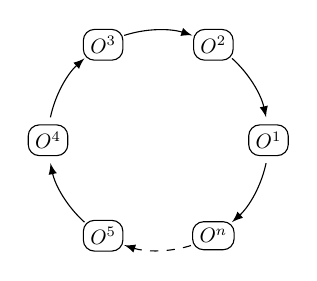
\begin{tikzpicture}[
circle/.style={
		scale=0.75,
		rounded corners,
		draw=black, 
		text centered,
		}
]

\def \n {6}
\def \m {4}
\def \radius {1.4cm}
\def \margin {12} % margin in angles, depends on the radius

\foreach \s in {1,...,\m}
{
  \node[draw, circle] at ({360/\n * (\s - 1)}:\radius) {$O^\s$};
  \draw[<-, >=latex] ({360/\n * (\s - 1)+\margin}:\radius) 
    arc ({360/\n * (\s - 1)+\margin}:{360/\n * (\s)-\margin}:\radius);
}

\node[draw, circle] at ({360/\n * 4}:\radius) {$O^5$};
  \draw[<-, dashed, >=latex] ({360/\n * 4+\margin}:\radius) 
    arc ({360/\n * 4+\margin}:{360/\n * (5)-\margin}:\radius);
    
\node[draw, circle] at ({360/\n * 5}:\radius) {$O^n$};
  \draw[<-, >=latex] ({360/\n * 5+\margin}:\radius) 
    arc ({360/\n * 5+\margin}:{360/\n * (6)-\margin}:\radius);


\end{tikzpicture}
\caption{环路撮合}
\label{fig:settlement}
\end{figurehere}
\end{center}

为了完成交易,LPSC会调用 \verb|TokenTransferDelegate|(代币转让代理)智能合约。引入这样一种代理机制使得升级协议智能合约变得更加简单,因为所有订单只需授权该代理,而不是协议的所有不同版本。

对于订单环路中的每个订单,根据执行情况,将会有一定数量的 \verb|tokenS| 支付给下一个或上一个订单。然后,根据矿工选择的收费模式支付矿工费。最后,一旦所有交易全部完成,便会发布一个 \verb|RingMined|(撮合完成)事件。

\subsubsection{发布事件\label{sec:events}}

路印协议发布事件,允许中继、订单浏览器和其他参与者尽可能高效地接收订单更新。发布的事件有:

\begin{itemize}
	\item \textbf{取消某一订单(OrderCancelled)}:某一特定订单已被取消。
	\item \textbf{取消某一交易对所有订单(OrdersCancelled)}:用户地址下某一交易对所有订单已全部取消。
	\item \textbf{取消所有订单(AllOrdersCancelled)}:用户地址下所有交易对订单已全部取消。
	\item \textbf{撮合完成(RingMined)}:某一订单环路已经成功撮合。该事件包含了环路内每笔代币转账的详细数据。
\end{itemize}


\section{LRx代币\label{sec:token}}
LRx是路印统一的代币符号。LRC是在以太坊网络上的路印代币,LRQ是在量子链网络上的路印代币,LRN是在NEO网络上的路印代币。随着路印不断在其他公有链上进行部署,未来我们还会引入其他类型的LRx代币。

\subsection{收费模式\label{sec:fee_model}} 
当用户创建订单时,他们会指定一定数量的LRx用来作为支付给矿工的手续费,一同连带的还有矿工能从该笔订单中分得的利润比例 (\verb|marginSplitPercentage|)。我们将其称之为分润比例。选择哪一种(手续费或分润比例)方式完全由矿工自主决定。

下图是一种分润比例展示图:

\begin{center}
\begin{figurehere}
\centering
\begin{tikzpicture}[
scale=1,
font=\normalfont,
classical/.style={thick,<->,shorten >=2pt,shorten <=2pt,>=stealth},
oneway/.style={->,dashed,shorten >=2pt,shorten <=2pt,>=stealth}
]
    % Draw axes
    \draw [->,thick] (0,1) node (yaxis) [above] {$$}
        |- (6.2,0) node (xaxis) [right] {$$};
        
    \draw
  	(4,0) coordinate (A)
  	(4,1) coordinate (A2)
  	(4.8,-0.6) coordinate (B)
  	(4.8,1) coordinate (B2)
  	(6,-0.6) coordinate (C)
  	(6,1) coordinate (C2);
  	
  	\fill [draw=none, fill=gray!20] 
    (4.8, 0) rectangle (6, 1);
    
  	\fill [draw=none, fill=gray!10] 
    (0, -0.6) rectangle (4.8, 0);

	\draw[thick] (0, -0.6) -- (0, 0.6) node[below]{$$};
  	\draw[thick, thin] (A) -- (A2) node[below]{$$};
  	\draw[thick, thin] (B) -- (B2) node[below]{$$};
  	\draw[thick] (C) node[below, xshift=0.5cm]{总买入量} -- (C2) ;
  	
  	\draw[classical] (0, 0.5) -> (4, 0.5) node[below]{$$};
  	\draw[classical] (4, 0.75) -> (4.8, 0.75) node[below]{$$};
%  	\draw[classical] (4.8, 0.5) -> (6, 0.5) node[below]{$$};
  	\draw[classical] (4, 0.25) -> (6, 0.25) node[below]{$$};

  	
  	\draw[oneway] (2, 1.2) node[above]{订单初始买入量} -- (2, 0.5);
  	\draw[oneway] (4.4, 2.2) node[above]{额外买入量} -- (4.4, 0.75);
  	\draw[oneway] (5.4, 1.6) node[above]{分润比例} -- (5.4, 1);
  	\draw[oneway] (5, -1.2) node[below]{利润} -- (5, 0.25);
  	\draw[oneway] (2.4, -1.2) node[below]{订单实际买入量} -- (2.4, -0.5);



\end{tikzpicture}
\caption{一种60\%的分润比例}
\label{fig:marginsplit}
\end{figurehere}
\end{center}

如果订单环路上的利润率太小,矿工将会选择LRx模式。相反,如果利润率足够大,以致于由此产生的分润比例远远超过LRx费用,则矿工会选择分润比例模式。然而,这里有另一个限制条件:当矿工选择分润比例模式时,他们必须向用户(订单创建者)支付一笔费用,数量相当于用户本应支付给矿工的LRx费用。这就将矿工选择分润比例模式的门槛提高到LRx费用模式的两倍,增强了选择LRx模式的倾向。这使得矿工能够在低利润率的环路订单上获得固定收入,以换取在较高利润率的环路订单上获得较少收入的平衡。对于这种收费模式,我们希望随着市场的发展和成熟,利润率较高的环路订单环将会减少,因此需要固定的LRx费用作为激励。


我们最终会得到下列图表:


\begin{center}
\begin{figurehere}
\centering
\begin{tikzpicture}[
font=\normalfont,
oneway/.style={->,dashed,shorten >=2pt,shorten <=2pt,>=stealth},
scale=1]
    % Draw axes
    \draw [<->,thick] (0,2.7) node (yaxis) [above] {$y$}
        |- (5,0) node (xaxis) [right] {$x$};
        
    \draw
  	(1,1) coordinate (A)
  	(2,1) coordinate (B);
  	
  	
  	\draw[thick] (B) -- (3.7,2.7);
  	\draw[dotted] (B) -- (2,0) node[below] {$2f$};
  	\draw[dotted] (A) -- (1,0) node[below] {$f$};
  	\draw[thick,color=gray!70] (0,0) -- (2.7,2.7);
  	\draw[thick] (0,1) node[left] {$f$}--(B) node[     ]{$$};
 	\draw[oneway] (4,1) node[right]{预期挖矿收益} -- (3, 2);


\end{tikzpicture}
\caption{路印收费模式}
\label{fig:feemodel}
\end{figurehere}
\end{center}

其中 $f$ 代表LRx费用, $x$ 代表分润比例, $y$ 代表挖矿收入。实线表示 $y=max(f, x-f)$;如果一笔订单的LRx费用为0,则用 $y=max(0, x - 0)$ 方程式表示。简单来讲,就是灰色实线代表 $y=x$。


由此带来的结果是: 
\begin{enumerate}
	\item 如果分润比例为0,矿工将会选择没什么吸引力的LRx费用模式,依然获得奖励。
	\item 如果LRx费用为0,便会出现灰色实线。此时矿工的收入将将呈一般线性模型。
	\item 当分润比例收入大于LRx费用模式的两倍时,矿工会选择分润比例模式,支付LRx给用户。
\end{enumerate}

需要注意的是,如果LRx费用不为零,不论矿工选择哪种费用模式,矿工与订单发起者之前总会发生LRx转账,矿工要么选择挣LRx费,要么就要将LRx费返还给订单发起者,然后收取分润比例费。

此外,矿工还将与钱包分享一定比例的费用。当用户通过一个钱包发起一笔订单并且最终成交时,会有一定比例的费用或分润比例奖励给钱包。尽管这种设置是模块化的,但我们依然可以根据需要设计独特的商业模式或应用,我们倾向于让钱包从矿工处中大约分得20\%-25\%的收益。因为钱包虽然是集成路印协议的主要目标,但其自身却只有很少或没有任何收入来源。

\subsection{去中心化自治}
从根本上讲,路印协议是一种社会协议,它依赖于成员之间的相互协作,从而有效实现某一目标。虽然这与一般密码经济协议并无不同,但实际上,它的有用性很大程度上受到同样的协调问题机制 \cite{vitalikgovernance}、严峻的触发平衡和有限理性的保护。为此,LRx代币的用途不仅仅只是支付费用,而且还用于协调各个网络参与者的财政激励。这种协调对于实现任何协议的广泛采用都是必要的,而且对于交换协议来说尤为重要,因为路印协议最终的成功与否在很大程度上取决于能否在一个健全的去中心化生态系统中提高流动性。

LRx代币将用于通过去中心化自治实现协议更新。未来,智能合约的更新将由代币持有者负责治理,从而确保连续性、安全性,并通过不兼容性降低流动性流失风险。考虑到智能合约一经部署便不可修改,dApp或终端用户可能会面临继续与被废弃的版本交互,且无法使用更新版协议的风险。升级能力是协议成功的关键,因为它必须适应市场和底层区块链的发展需要。LRx股东的去中心化治理将允许协议智能合约在不影响dApp、终端用户,或过度依赖智能合约提取的的情况下实现升级。LRx代币发行总量是固定的,以LRC为例,一定比例的代币归路印基金会所有,一定比例的代币被用作支持社区发展的资金。

然而,LRx代币持有者并不是唯一的掌握路印协议发展方向的股东:中继/环路矿工、钱包、开发人员和其他参与者也是整个生态系统的一个组成部分,路印协议的发展也必须听取他们的意见和建议。事实上,鉴于这些参与者不需要持有任何LRx代币来履行各自的角色(因为路印协议中不存在传统的卖方/买方和做市商角色,初始代币准备金并不是强制性的),我们必须通过其他方法来满足他们的利益。此外,“简单”的以代币为基础的投票,无论是在链上还是在链下,都是不完美的,会带来分歧,因为低投票率和代币过渡集中会带来风险。因此,我们的目标是实现一个构建在层中的治理模型,做到在达成共识的基础上建立一套标准决策过程。我们可以借助协调机构来收集各个参与者群体,也许还可以是预先确定的协议联络点的不同声音。随着这一成果的实现,路印基金会必然会逐步从协议开发人员演变为协议管理员。

\section{欺诈和攻击保护}

\subsection{防范抢先交易\label{sec:dual_authoring}}

在去中心化交易中,抢先交易指有人试图复制另一节点的交易方案,撮合未成交交易池(mempool)已外的交易,可以通过指定较高的交易费用(油费)来实现。在路印协议中存在的抢先交易(以及其他订单撮合协议)主要为订单偷窃:抢先交易者从未成交的环路撮合交易中偷取一个或多个订单。具体到路印便是:抢先交易者从未成交交易中偷取整个订单环路。


当提交的环路交易(submitRing)没有被确认并且仍然在未成交交易池中时,这样的交易很容易被人发现,环路偷窃者可以轻而易举地把自己的地址(the \verb|filcherAddress|)替换成矿工地址(\verb|minerAddress|)对交易负载重新签名,接着 \verb|filcherAddress| 就取代了订单环路签名。偷窃者可以设置更高的油费,提交一笔新的交易,吸引矿工优先撮合他提交的新交易,而不是原来提交的环路交易。

面对这一问题,我们之前提出的解决方案存在一些重要缺陷:它需要更多的交易支持,因此矿工会消耗更多的油费,同时撮合一个环路要花费至少双倍的区块时间。我们的新的“双重授权”(Dual Authoring)解决方案包括为订单设置两个级别的授权机制:一个用于结算,另一个用于挖矿。


双重授权流程:

\begin{enumerate}

	\item 对于每个订单,钱包软件将生成随机的公钥/私钥对,并将密钥对加入订单的JSON片段中。(另一种方法是使用公钥派生的地址代替公钥本身,以减小字节大小,我们使用 \verb|authAddr| 来表示这样一个派生地址, \verb|authKey| 表示 \verb|authAddr| 的配对私钥)。

	\item 用订单中除 \verb|r|, \verb|v|, \verb|s|, 和 \verb|authKey| 以外所有的字段计算出订单的哈希值,然后使用订单所有者的的私钥(不是 \verb|authKey|)进行签名。

	\item 钱包会将订单和 \verb|authKey| 一起发送给中继进行撮合。矿工将验证 \verb|authKey| 和 \verb|authAddr| 是否正确配对,且订单的签名对订单所有者地址有效。 

	\item 当发现一个新提交的订单环路时,矿工将使用每个订单的 \verb|authKey| 对环路哈希、 \verb|minerAddress| 和所有挖矿参数进行签名。如果一个环路包含 $n$ 个订单,\verb|authKey|s 就将产生 $n$ 个签名,我们称这些签名为 \verb|authSignature|s。矿工也许还需要使用 \verb|minerAddress| 的私钥对环路哈希及所有挖矿参数进行签名。

	\item 矿工使用所有参数和额外的 \verb|authSignature|s 调用submitRing函数。请注意,\verb|authKey|s 不是链上交易的一部分,因此除矿工本身没有任何人知道。

	\item 路印协议现在会对每个订单相应的 \verb|authAddr| 验证其 \verb|authSignature|,如果发现任何丢失或无效的 \verb|authSignature|,就会拒绝该环路的交易。
 
\end{enumerate}

由此带来的结果是:

\begin{itemize}

	\item  订单的签名(通过订单所有者地址私钥签署)保证订单和 \verb|authAddr| 不被修改。
	\item  矿工的签名(由 \verb|minerAddress| 的私钥签署),如果提供,保证没有人可以窃取他/她的身份进行环路撮合。
	\item  \verb|authSignature|s 保证整个环路都不能被篡改,包括 \verb|minerAddress|,因此订单是无法被窃取的。

\end{itemize}

双重授权可以防止环路偷窃和订单偷窃,同时确保订单撮合可以在一个交易中完成。另外,双重授权还为中继的订单共享提供了两种方式:不匹配共享和可匹配共享。默认情况下,路印的运作模式属于OTC,并且只支持限价订单,这意味着订单的时间戳将被忽略,意味着抢先交易虽然确实会影响交易的执行与否,但对交易的实际成交价格没有任何影响。

\section{其他攻击}

\subsection{Sybil或DOS攻击}
恶意用户——以自身身份或伪造身份——可以通过发送大量小额订单来攻击路印节点。然而,由于我们允许节点根据自身标准拒绝订单——它们可能会选择隐藏或公开这些标准——大多数这样的订单将因为匹配时不能产生令人满意的利润而被拒绝。通过授权中继来决定如何管理订单,我们认为大规模的小订单攻击并不是一种威胁。

\subsection{余额不足订单攻击}
恶意用户可以对订单值为非零但其地址余额实际为零的订单进行签名和广播。节点监视并注意到某些订单的实际余额为零后,相应地更新这些订单状态,然后丢弃它们。虽然节点必须花费时间更新订单的状态,但也可以选择通过例如将地址列入黑名单和删除相关订单的方式将工作量最小化。

\section{总结}

路印协议致力于成为去中心化交易服务的基础层。这一过程将会对人们如何交易资产和价值产生深刻影响。货币作为一种中间商品,促进或替代了物物交换,解决了“双方需求的巧合匹配”问题 \cite{unenumerated2006},即双方必须给予彼此不同的商品或服务。同样,路印协议旨在通过使用环路撮合来更容易地完成交易,从而消除我们对交易对中需求重合的依赖。这对于社会和市场如何交易代币/传统资产以及其他更广泛的事物都很有意义。事实上,正如去中心化加密数字货币对国家对货币的控制构成威胁一样,一种能够大规模撮合交易者(消费者/生产者)的组合协议,理论上也会对货币概念本身构成威胁。

路印协议带来的好处包括:

\begin{itemize}
	\item 链下订单管理与链上撮合结合在一起意味着没有因为安全考虑而牺牲任何性能。
	\item 环路撮合和订单分享带来了更大的流动性。
	\item 双重授权方案解决了当今所有DEX和其用户所面临的极为有害的抢先交易问题。
	\item 免费而公开的智能合约使任何dApp都可以在路印协议上构建应用或与协议本身进行交互。
	\item 运营商之间形成的统一标准提高了网络效率和终端用户体验。
	\item 在管理订单表和广播订单时的网络灵活性更强。
	\item 降低准入门槛意味着节点加入网络和终端用户所需的费用更低。
	\item 实现了用户钱包间直接的匿名交易。
\end{itemize}

\section{致谢}
在这里,我们想由衷地感谢我们的导师、顾问以及广大路印社区参与者,感谢他们如此热情和慷慨地用自身学识对白皮书中的内容提出意见。在此,我们要尤其感谢中国分布式总账基础协议联盟(ChinaLedger)白硕;阚海滨博士;Alex  Cheng,达鸿飞;曹寅;吴小川;Zhen  Wang、于伟、段念、肖军、钱江、向江旭、郭一鹏、李大海、Kelvin Long、夏华夏、马俊和Encephalo Path对本项目的评审建议和意见。


\bibliography{whitepaper}
\bibliographystyle{unsrt}


\end{multicols}


\begin{appendices}

\section{以太坊网络上的路印协议\label{app:protocol_ethereum}}

\subsection{智能合约}

\begin{center}
\begin{figurehere}
\centering
\begin{tikzpicture}
[node distance = 1cm, auto,font=\footnotesize,
% STYLES
every node/.style={node distance=3cm},
% The comment style is used to describe the characteristics of each force
comment/.style={rectangle, inner sep= 7pt, text width=4cm, node distance=0.25cm, font=\scriptsize\sffamily},
% The force style is used to draw the forces' name
force/.style={rectangle, draw, fill=black!10, inner sep=5pt, text width=4cm, text badly centered, minimum height=1.2cm, font=\normalfont}] 

% Draw forces
\node [force] (impl) {路印协议执行};
\node [force, dashed, above of=impl] (protocol_interface) {路印协议};
\node [force, left=1cm of impl] (nameregistry) {名称注册};
\node [force, right=1cm of impl] (tokenregistry) {代币注册};
\node [force, below of=impl] (delegate) {代币转让代理};
\node [force, left=1cm of delegate] (multisig) {可转让多重签名};

%%%%%%%%%%%%%%%
% Change data from here

% impl
\node [comment, below=0.25 of impl] (comment-impl) {- 验证订单环路\\
- 转让代币用于撮合\\
- 发布事件};

% nameregistry
\node [comment, below=0.25cm of nameregistry]{- 注册钱包和中继};

% protocol_interface
\node [comment, below=0.25 of protocol_interface](comment-interface) {- 定义交互界面和事件};

% tokenregistry
\node [comment, below=0.25 of tokenregistry] {- 注册ERC20/ERC223代币};

% delegate
\node [comment, below=0.25 of delegate] {- 代表用户转让代币};

% PUBLIC POLICIES
\node [comment, text width=3cm, below=0.25 of multisig] {- 激活多重签名所有权};

%%%%%%%%%%%%%%%%

% Draw the links between forces
\path[->,thick] 
(comment-interface) edge (impl)
(nameregistry) edge (impl)
(tokenregistry) edge (impl)
(delegate) edge (comment-impl);

\end{tikzpicture} 
\caption{智能合约}
\label{fig:smartcontracts}
\end{figurehere}
\end{center}

\subsection{智能合约部署情况}

下述智能合约已经在以太坊主网上部署完毕:
\begin{itemize}
\item LRC: \verb|0xEF68e7C694F40c8202821eDF525dE3782458639f|
\item TokenRegistry: \verb|0xa21c1f2AE7f721aE77b1204A4f0811c642638da9|
\item TokenTransferDelegate: \verb|0xc787aE8D6560FB77B82F42CED8eD39f94961e304|
\item NameRegistry: \verb|0x0f3Dce8560a6010DE119396af005552B7983b7e7|
\item LoopringProtocolImpl: \verb|0xc80BbAb86cED62CF795619A357581FaF0cB46511|
\item TransferableMultsig: \verb|0x7421ad9C880eDF007a122f119AD12dEd5f7C123B|
\end{itemize}

\end{appendices}
\end{document}
